% =============================================================================
% Paper IEEE (conference) - Visión por Computadora II - CEIA - FIUBA
% Compilar desde esta carpeta:  latexmk -pdf main.tex
% (o con la receta "latexmk" de LaTeX Workshop en VS Code)
% =============================================================================
\documentclass[conference,a4paper]{IEEEtran}
\IEEEoverridecommandlockouts

% --- Idioma y codificación ---------------------------------------------------
\usepackage[utf8]{inputenc}
\usepackage[T1]{fontenc}
\usepackage[spanish,es-tabla,es-nodecimaldot]{babel}

% --- Paquetes -----------------------------------------------------------------
\usepackage{cite}
\usepackage{amsmath,amssymb,amsfonts}
\usepackage{graphicx}
\usepackage{booktabs}
\usepackage{multirow}
\usepackage{siunitx}
\usepackage{xcolor}
\usepackage{url}

\graphicspath{{figures/}}
\sisetup{output-decimal-marker={,}}

% Nombres en español para elementos propios de IEEEtran
\renewcommand{\IEEEkeywordsname}{Palabras clave}

% Marcador visible para contenido pendiente (borrar antes de entregar)
\newcommand{\pendiente}[1]{\textcolor{red}{\textbf{[PENDIENTE:} #1\textbf{]}}}

% Salto de línea entre bloques de autores (grilla 2x2 en lugar de 4 columnas)
\makeatletter
\newcommand{\linebreakand}{%
  \end{@IEEEauthorhalign}\hfill\mbox{}\par\mbox{}\hfill\begin{@IEEEauthorhalign}}
\makeatother

\begin{document}

\title{Clasificación de enfermedades en hojas de plantas mediante transfer learning:
comparación de arquitecturas livianas y explicabilidad con Grad-CAM}

\author{
\IEEEauthorblockN{BETTIG, Santiago Federico}
\IEEEauthorblockA{\textit{CEIA - FIUBA} \\
\textit{Universidad de Buenos Aires}\\
Buenos Aires, Argentina \\
santiagofbettig@gmail.com}
\and
\IEEEauthorblockN{DIEGUEZ, Manuel}
\IEEEauthorblockA{\textit{CEIA - FIUBA} \\
\textit{Universidad de Buenos Aires}\\
Buenos Aires, Argentina \\
manueldieguezw@gmail.com}
\linebreakand
\IEEEauthorblockN{RUBIOLO, Pedro Ignacio}
\IEEEauthorblockA{\textit{CEIA - FIUBA} \\
\textit{Universidad de Buenos Aires}\\
Buenos Aires, Argentina \\
rubiolopedroignacio@gmail.com}
\and
\IEEEauthorblockN{TOLOTTO, Lourdes}
\IEEEauthorblockA{\textit{CEIA - FIUBA} \\
\textit{Universidad de Buenos Aires}\\
Buenos Aires, Argentina \\
tolottolourdes2309@gmail.com}
}

\maketitle

\begin{abstract}
El diagnóstico temprano de enfermedades en los cultivos depende de la inspección visual de
especialistas, un recurso escaso para muchos productores. En este trabajo desarrollamos un
prototipo de clasificación de 15 clases de hojas sanas y enfermas de pimiento, papa y tomate
del dataset PlantVillage, basado en arquitecturas livianas preentrenadas en ImageNet y
entrenado íntegramente en CPU. Para evitar la fuga de datos, particionamos el dataset de forma
estratificada y agrupada por imágenes casi duplicadas. Comparamos cuatro backbones mediante
linear probe y aplicamos fine-tuning parcial a MobileNetV3-Small y EfficientNet-B0, con y sin
data augmentation. EfficientNet-B0 con augmentation alcanza un macro-F1 de 0,993 en test, con
una latencia de 17,5\,ms por imagen en CPU. El augmentation no modifica el desempeño en el test
original, pero es decisivo ante perturbaciones: con desenfoque, el macro-F1 cae 0,23 sin
augmentation y solo 0,013 con él. Un análisis cuantitativo con Grad-CAM muestra que el 65,7\,\%
de la activación recae sobre la hoja, que ocupa el 40,2\,\% de la imagen, y que los errores se
deben a síntomas ambiguos más que a una atención desviada hacia el fondo. Sin embargo, sobre
imágenes de campo del dataset PlantDoc el accuracy cae al 36,7\,\%. Estos resultados indican
que un desempeño cercano al 100\,\% en PlantVillage no garantiza la utilidad del modelo en
condiciones reales.
\end{abstract}

\begin{IEEEkeywords}
clasificación de imágenes, enfermedades de plantas, transfer learning, PlantVillage, EfficientNet, MobileNetV3, Grad-CAM
\end{IEEEkeywords}

\section{Introducción}
\label{sec:introduccion}

Las plagas y enfermedades de los cultivos son una de las principales amenazas para la
seguridad alimentaria. Una evaluación global sobre cinco cultivos básicos estimó que las
pérdidas de rendimiento atribuibles a patógenos y plagas alcanzan, en el caso de la papa,
un 17,2\,\% en promedio (8,1--21,0\,\% según la región), y que las pérdidas más altas se
concentran en regiones con déficit de alimentos~\cite{savary2019burden}. El manejo de estas
enfermedades depende de un diagnóstico temprano, que todavía se apoya mayormente en la
inspección visual realizada por especialistas: un recurso escaso y costoso, sobre todo para
productores pequeños y alejados de los centros técnicos.

El aprendizaje profundo y la masificación de los teléfonos inteligentes abrieron la
posibilidad de automatizar ese diagnóstico a partir de una fotografía de la hoja. El dataset
PlantVillage~\cite{hughes2015plantvillage} fue el punto de partida de esta línea: sobre
54\,306 imágenes de 14 especies, una red convolucional alcanzó un 99,35\,\% de accuracy en
un conjunto de test separado~\cite{mohanty2016using}. Sin embargo, el mismo trabajo reportó
que el accuracy caía al 31,4\,\% sobre imágenes obtenidas de otras fuentes. Estudios
posteriores mostraron que PlantVillage contiene sesgos de captura que un modelo puede
explotar (por ejemplo, un clasificador entrenado con solo 8 píxeles del fondo alcanza un
49\,\% de accuracy~\cite{noyan2022uncovering}) y propusieron conjuntos de imágenes tomadas
en condiciones reales, como PlantDoc~\cite{singh2020plantdoc}. En consecuencia, un
accuracy cercano al 100\,\% en PlantVillage no garantiza por sí solo un modelo útil en el
campo, y su evaluación debe complementarse con controles de fuga de datos, explicabilidad y
pruebas fuera de la distribución de entrenamiento.

% --- Caso real de aplicación (<= 7 años). Propuesta: PlantVillage Nuru. ---------------
Un caso real que ilustra tanto el potencial como esta brecha es PlantVillage Nuru, una
aplicación móvil que ejecuta sin conexión un modelo de detección de síntomas foliares en
mandioca~\cite{ramcharan2019mobile}. En una evaluación de campo en Tanzania, Nuru alcanzó un
65\,\% de accuracy en el diagnóstico de enfermedades virales, por encima de los extensionistas
agrícolas (40--58\,\%) y de los productores (18--31\,\%), y llegó al 74--88\,\% cuando el
diagnóstico combinaba seis hojas por planta~\cite{mrisho2020accuracy}. Estos resultados
muestran que un modelo liviano ejecutado en el teléfono puede aportar valor real, pero
también que el desempeño en el campo es muy inferior al que se obtiene en el laboratorio.

En este trabajo desarrollamos un prototipo de clasificación de enfermedades foliares en
tres cultivos de importancia hortícola (pimiento, papa y tomate), con 15 clases que incluyen
hojas sanas y enfermas de PlantVillage. Partimos de modelos preentrenados en ImageNet y
priorizamos arquitecturas livianas (MobileNetV3~\cite{howard2019searching} y
EfficientNet-B0~\cite{tan2019efficientnet}), compatibles con una inferencia en CPU o en
dispositivos móviles. Las contribuciones principales son:
\begin{itemize}
  \item un protocolo de partición estratificada y agrupada por imágenes casi duplicadas, que
        reduce la fuga de datos entre entrenamiento y test;
  \item una comparación sistemática entre \emph{linear probe} y \emph{fine-tuning} parcial de
        distintos backbones, con y sin data augmentation;
  \item un análisis cuantitativo de explicabilidad con Grad-CAM~\cite{selvaraju2017gradcam},
        que mide qué fracción de la atención del modelo recae sobre la hoja y no sobre el fondo;
  \item una evaluación de robustez ante perturbaciones de la imagen y sobre datos externos a
        PlantVillage, junto con la medición del costo de inferencia en CPU.
\end{itemize}

El resto del trabajo se organiza de la siguiente manera: la Sección~\ref{sec:metodologia}
describe los datos, la partición, las arquitecturas y el protocolo experimental; la
Sección~\ref{sec:resultados} presenta y analiza los resultados; y la
Sección~\ref{sec:conclusiones} resume las conclusiones y las líneas de trabajo futuro.

\section{Metodología, diseño y desarrollo}
\label{sec:metodologia}

\subsection{Dataset}
\label{subsec:dataset}
Utilizamos el subconjunto de PlantVillage~\cite{hughes2015plantvillage} correspondiente a
pimiento, papa y tomate: 20\,638 imágenes RGB de $256\times256$ píxeles distribuidas en 15
clases (12 enfermedades y 3 clases de hoja sana). Las imágenes fueron tomadas en condiciones
de laboratorio, con una única hoja centrada sobre un fondo uniforme. El dataset está
desbalanceado (Fig.~\ref{fig:datos}a): la clase mayoritaria (virus del rizado amarillo del
tomate, TYLCV) tiene 3\,208 imágenes y la minoritaria (papa sana) 152, una relación de 21:1.
Las hojas sanas representan el 15,6\,\% del total. Por este desbalance adoptamos el macro-F1
como métrica principal.

\begin{figure}[t]
\centering
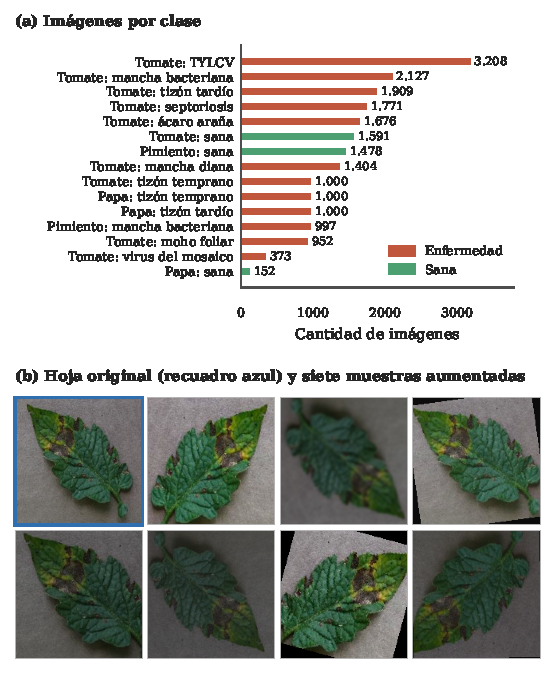
\includegraphics[width=\columnwidth]{metodologia_datos.pdf}
\caption{(a) Cantidad de imágenes por clase en el subconjunto de PlantVillage utilizado.
(b) Una hoja de entrenamiento (tizón temprano del tomate) y siete muestras generadas por el
pipeline de data augmentation usado en el fine-tuning ($160\times160$).}
\label{fig:datos}
\end{figure}

\subsection{Partición de datos y control de fuga}
\label{subsec:split}
PlantVillage incluye varias fotografías de una misma hoja, por lo que una partición aleatoria
puede ubicar imágenes casi idénticas en entrenamiento y en test e inflar las métricas. Para
detectarlas calculamos un hash criptográfico (MD5) de cada archivo y un hash perceptual
(dHash de 64 bits). Encontramos 28 imágenes en 14 grupos de duplicados, todos con etiquetas
consistentes. Luego realizamos una partición estratificada por clase y \emph{agrupada} por
dHash (\texttt{StratifiedGroupKFold}, semilla fija), de modo que las imágenes de un mismo
grupo caen siempre en el mismo subconjunto. El resultado es una partición
71,4/14,3/14,3\,\% (14\,740 imágenes de entrenamiento, 2\,949 de validación y 2\,949 de
test), sin grupos compartidos entre subconjuntos. Esta partición se versiona en el
repositorio y es la misma para todos los experimentos. Como el dHash no es invariante a
rotaciones, este control no elimina la fuga entre fotografías rotadas de una misma hoja; lo
consideramos una limitación del estudio.

\subsection{Preprocesamiento y data augmentation}
\label{subsec:augmentation}
Las imágenes se normalizan con la media y el desvío de ImageNet, que son los usados para
preentrenar los backbones. Validación y test usan siempre un preprocesamiento determinístico
(solo redimensionado). El data augmentation se aplica únicamente en entrenamiento y combina
recortes aleatorios (escala 0,6 - 1,0), volteos horizontales y verticales, rotaciones de hasta
$\pm30^\circ$ ($p=0{,}5$), variaciones moderadas de color (brillo y contraste $\pm30$\,\%,
saturación $\pm20$\,\%, tono $\pm0{,}03$) y desenfoque gaussiano ($p=0{,}2$)
(Fig.~\ref{fig:datos}b). Las hojas no
tienen una orientación canónica, por lo que las transformaciones geométricas son válidas. En
cambio, las variaciones de color se limitaron porque el color es en sí mismo una señal
diagnóstica (clorosis, necrosis).

\subsection{Arquitecturas y estrategia de transferencia}
\label{subsec:arquitecturas}
Elegimos backbones preentrenados en ImageNet con distintos compromisos entre costo y
capacidad: MobileNetV3-Small y MobileNetV3-Large~\cite{howard2019searching},
EfficientNet-B0~\cite{tan2019efficientnet} y, como referencia sin optimización para
dispositivos móviles, ResNet18. Como el entrenamiento se realizó íntegramente en CPU, seguimos
una estrategia en dos etapas:
\begin{enumerate}
  \item \textbf{Linear probe}: con el backbone congelado, extraemos una única vez los
        embeddings de todas las imágenes a $224\times224$ y entrenamos sobre ellos una capa
        lineal. Esta etapa, de pocos segundos por modelo, mide la calidad de las
        representaciones de ImageNet para este dominio y permite comparar las cuatro
        arquitecturas a bajo costo. También evaluamos una entropía cruzada ponderada por la
        frecuencia inversa de cada clase.
  \item \textbf{Fine-tuning parcial}: para las dos arquitecturas con mayor macro-F1 en
        validación en la etapa anterior (EfficientNet-B0 y MobileNetV3-Small, esta última
        además la de menor costo), reemplazamos el clasificador y
        reentrenamos las últimas etapas del backbone (6 bloques en MobileNetV3-Small y 3 en
        EfficientNet-B0, con 1,39\,M y 3,17\,M parámetros entrenables, respectivamente). Las
        BatchNorm de las etapas congeladas se mantienen en modo evaluación para no alterar sus
        estadísticas. Cada arquitectura se entrena con y sin data augmentation, en un diseño
        $2\times2$ en el que todo lo demás (semilla, partición, resolución, optimizador y
        número de épocas) permanece fijo.
\end{enumerate}

\subsection{Protocolo de entrenamiento y métricas}
\label{subsec:entrenamiento}
La Tabla~\ref{tab:config} resume los hiperparámetros de ambas etapas. Para reducir el costo
en CPU, el fine-tuning se realiza a $160\times160$ píxeles. En las dos etapas, la mejor época
se elige por macro-F1 en validación, y el conjunto de test se evalúa una única vez con el
modelo seleccionado. Reportamos accuracy, balanced accuracy y macro-F1, además del F1 por
clase y la matriz de confusión para el análisis de errores. Como métricas de costo
registramos el tiempo de entrenamiento, el número de parámetros y la latencia de inferencia
en CPU.

\begin{table}[t]
\centering
\caption{Configuración de entrenamiento}
\label{tab:config}
\setlength{\tabcolsep}{4pt}
\begin{tabular}{@{}lcc@{}}
\toprule
 & \textbf{Linear probe} & \textbf{Fine-tuning} \\
\midrule
Resolución de entrada      & $224\times224$          & $160\times160$ \\
Capas entrenadas           & capa lineal             & últimas etapas + cabeza \\
Optimizador                & AdamW                   & AdamW \\
Learning rate\textsuperscript{a} & $3\times10^{-3}$  & $10^{-3}$ / $3\times10^{-4}$ \\
Weight decay               & $10^{-3}$               & $10^{-4}$ \\
Scheduler                  & coseno                  & coseno \\
Batch / épocas             & 256 / 60                & 32 / 8 \\
Pérdida                    & CE y CE ponderada       & CE \\
Selección del modelo       & \multicolumn{2}{c}{máximo macro-F1 en validación} \\
\bottomrule
\multicolumn{3}{@{}l}{\footnotesize \textsuperscript{a}En fine-tuning: cabeza / backbone.}
\end{tabular}
\end{table}

\subsection{Explicabilidad con Grad-CAM}
\label{subsec:gradcam}
Para auditar en qué regiones de la imagen se basa el mejor modelo aplicamos
Grad-CAM~\cite{selvaraju2017gradcam} sobre la última capa convolucional del backbone (un mapa
de $5\times5$ a la resolución de entrada), calculado para la clase predicha. Además del
análisis visual, cuantificamos la atención del modelo sobre todo el conjunto de test. Para
cada imagen segmentamos la hoja con un umbral de Otsu sobre el canal de saturación (el fondo
de laboratorio es poco saturado), seguido de limpieza morfológica. Con la máscara $M$
resultante y el mapa Grad-CAM normalizado $L$ calculamos la fracción de la activación que recae 
sobre la hoja:
\begin{equation}
  E_{\text{hoja}} = \frac{\sum_{i,j} L_{ij}\,M_{ij}}{\sum_{i,j} L_{ij}},
\end{equation}
Como un mapa uniforme obtendría un valor igual al área relativa de la hoja, también reportamos 
el cociente entre $E_{\text{hoja}}$ y esa área (mayor que 1 si la atención se concentra en la 
hoja más de lo esperable por azar). Por último, aplicamos el \emph{pointing game}, que mide 
el porcentaje de imágenes cuyo máximo de activación cae dentro de la hoja. Estas métricas 
permiten detectar si el modelo explota el fondo, un sesgo conocido de PlantVillage~\cite{noyan2022uncovering}, 
en lugar de los síntomas.

\subsection{Evaluación de robustez y con datos externos}
\label{subsec:robustez_metodo}
\pendiente{Perturbaciones aplicadas al test (tipos y niveles), dataset externo utilizado,
mapeo de clases y protocolo de evaluación.}

\section{Resultados experimentales y análisis}
\label{sec:resultados}

% Figuras de ancho completo: se declaran al inicio para que LaTeX las ubique arriba de una página.
\begin{figure*}[t]
\centering
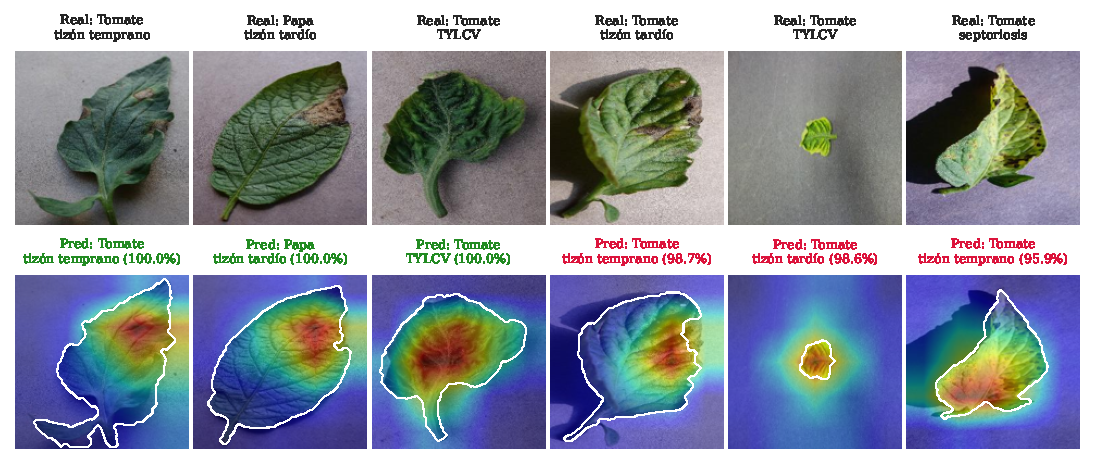
\includegraphics[width=\textwidth]{gradcam_ejemplos.pdf}
\caption{Grad-CAM del modelo EfficientNet-B0 con augmentation sobre imágenes de test. Las tres
columnas de la izquierda muestran aciertos típicos (imagen con la mediana de $E_{\text{hoja}}$
dentro de su clase) y las tres de la derecha, los errores con mayor confianza. El contorno
blanco indica la máscara de la hoja usada para calcular $E_{\text{hoja}}$.}
\label{fig:gradcam_ejemplos}
\end{figure*}

\subsection{Comparación de backbones (linear probe)}
\label{subsec:res_linear_probe}
La Tabla~\ref{tab:linear_probe} resume el desempeño de una capa lineal entrenada sobre los
embeddings congelados de cada backbone. Sin modificar ningún peso preentrenado, todas las
arquitecturas superan el 94\,\% de macro-F1 en test, lo que confirma que las representaciones
de ImageNet transfieren bien a este dominio. Las arquitecturas diseñadas para dispositivos
móviles superan a ResNet18 (macro-F1 0,960 contra 0,942) a pesar de tener entre 4 y 12 veces
menos parámetros. Entre ellas, las diferencias en test son menores a 0,002, del orden de la
variabilidad entre validación y test: EfficientNet-B0 obtiene el mayor macro-F1 en validación
y MobileNetV3-Small, uno prácticamente igual con una extracción 3,3 veces más rápida. La
entropía cruzada ponderada no mostró un beneficio consistente: modificó el macro-F1 en test
entre $-0{,}007$ y $+0{,}004$ según el modelo, por lo que no la utilizamos en el fine-tuning.

\begin{table}[t]
\centering
\caption{Linear probe sobre backbones congelados (entropía cruzada sin ponderar)}
\label{tab:linear_probe}
\setlength{\tabcolsep}{4pt}
\begin{tabular}{@{}lccccc@{}}
\toprule
\textbf{Backbone} & \textbf{Parám.} & \textbf{Extracción} & \multicolumn{2}{c}{\textbf{Macro-F1}} & \textbf{Bal. acc.} \\
\cmidrule(lr){4-5}
 & (M) & (img/s) & val & test & test \\
\midrule
MobileNetV3-Small & 0,9  & 208,6 & 0,972          & 0,960          & 0,962 \\
MobileNetV3-Large & 3,0  & 91,1  & 0,967          & 0,960          & 0,957 \\
EfficientNet-B0   & 4,0  & 62,7  & \textbf{0,974} & 0,959          & 0,961 \\
ResNet18          & 11,2 & 55,4  & 0,943          & 0,942          & 0,941 \\
\bottomrule
\end{tabular}
\end{table}

\subsection{Fine-tuning con y sin data augmentation}
\label{subsec:res_finetuning}
El fine-tuning parcial mejora de forma sustancial el linear probe
(Tabla~\ref{tab:finetuning}). El macro-F1 en test pasa de 0,960 a 0,986 en MobileNetV3-Small
y de 0,959 a 0,994 en EfficientNet-B0, lo que equivale a reducir la fracción de error
($1-\text{macro-F1}$) un 65\,\% y un 85\,\%, respectivamente. Adaptar las últimas etapas del
backbone resulta, entonces, mucho más determinante que la elección de la arquitectura en la
etapa de linear probe. EfficientNet-B0 supera a MobileNetV3-Small en todas las métricas, con
la mitad de errores, pero su entrenamiento demora tres veces más.

El data augmentation no mejoró el desempeño en el test de PlantVillage: las diferencias
entre las corridas con y sin augmentation son de a lo sumo 0,002 en macro-F1 (6 imágenes de
2\,949), un margen que no consideramos significativo con una sola semilla. Sí se observa su
efecto regularizador: sin augmentation, EfficientNet-B0 termina con una pérdida de
entrenamiento de 0,003 frente a 0,016 en validación (memoriza el conjunto de entrenamiento),
mientras que con augmentation la pérdida de entrenamiento (0,038) queda por encima de la de
validación (0,019). Como el test proviene de la misma distribución que el entrenamiento, es
esperable que el beneficio del augmentation aparezca recién ante condiciones de captura
distintas (Secciones~\ref{subsec:res_robustez} y~\ref{subsec:res_externos}). Por último, en
las cuatro corridas el macro-F1 de validación todavía crecía en la última época, por lo que
un entrenamiento más largo podría mejorar levemente estos valores.

\begin{table}[t]
\centering
\caption{Fine-tuning parcial a $160\times160$ (8 épocas, CPU)}
\label{tab:finetuning}
\setlength{\tabcolsep}{3.5pt}
\begin{tabular}{@{}lcccccc@{}}
\toprule
\textbf{Modelo} & \textbf{Aug.} & \textbf{Parám.} & \textbf{F1 val} & \textbf{F1 test} & \textbf{Errores} & \textbf{Tiempo} \\
 & & entren. (M) & & & test & (min) \\
\midrule
MobileNetV3-S   & no & 1,39 & 0,990          & 0,986          & 24          & 10,7 \\
MobileNetV3-S   & sí & 1,39 & 0,987          & 0,986          & 30          & 10,6 \\
EfficientNet-B0 & no & 3,17 & 0,995          & \textbf{0,994} & \textbf{11} & 33,8 \\
EfficientNet-B0 & sí & 3,17 & \textbf{0,995} & 0,993          & 17          & 32,4 \\
\bottomrule
\end{tabular}
\end{table}

\subsection{Análisis por clase y de errores}
\label{subsec:res_errores}
Con el modelo seleccionado (EfficientNet-B0 con augmentation, el de mayor macro-F1 en
validación), todas las clases superan un F1 de 0,975. Las más bajas son tizón temprano del
tomate (0,975) y papa sana (0,976). Esta última es la clase con menor F1 en tres de las
cuatro corridas, lo que es coherente con que sea la clase minoritaria (21 imágenes de test).
De los 17 errores, 16 ocurren entre enfermedades de una misma especie y solo uno confunde una
hoja sana con una enferma. Las confusiones más frecuentes se dan entre enfermedades del
tomate con síntomas visualmente parecidos: tizón temprano contra tizón tardío, y mancha diana
contra ácaro araña o moho foliar. Estos mismos pares ya aparecían como los principales
errores del linear probe, lo que sugiere una ambigüedad propia de los síntomas más que una
limitación de un modelo en particular.

\subsection{Explicabilidad (Grad-CAM)}
\label{subsec:res_gradcam}
% Nota: Grad-CAM se calculó sobre un reentrenamiento de EfficientNet-B0 con augmentation
% (branch gradcam). Actualizar al unificar los resultados en main.
El análisis de Grad-CAM se realizó sobre un reentrenamiento del mismo modelo (macro-F1 en
test de 0,994; 13 errores). En el conjunto de test completo, el 67,8\,\% de la activación
recae sobre la hoja, que ocupa en promedio el 40,2\,\% de la imagen: la atención está
1,77 veces más concentrada en la hoja de lo que se esperaría por azar. Además, el máximo de
activación cae dentro de la hoja en el 97,0\,\% de las imágenes (Fig.~\ref{fig:energia_hoja}).
Los aciertos de la Fig.~\ref{fig:gradcam_ejemplos} muestran que el modelo se enfoca en las
lesiones necróticas y en las zonas cloróticas.

\begin{figure}[t]
\centering
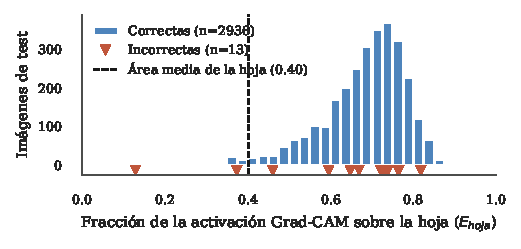
\includegraphics[width=\columnwidth]{gradcam_energia_hoja.pdf}
\caption{Distribución de $E_{\text{hoja}}$ (fracción de la activación Grad-CAM sobre la hoja)
en las 2\,949 imágenes de test. Los triángulos marcan los 13 errores; la línea punteada, el
área media que ocupa la hoja.}
\label{fig:energia_hoja}
\end{figure}

Los errores no se explican por una atención desviada hacia el fondo: su $E_{\text{hoja}}$
medio (0,63) y su \emph{pointing game} (92\,\%) son apenas menores que los de los aciertos
(0,68 y 97\,\%). Es decir, el modelo mira la hoja pero interpreta mal síntomas ambiguos. La
excepción es una hoja de TYLCV de tamaño muy reducido, en la que la activación se extiende
sobre el fondo (Fig.~\ref{fig:gradcam_ejemplos}, cuarta columna). Las clases con menor
$E_{\text{hoja}}$ son el virus del mosaico (0,54) y el tizón tardío del tomate (0,55), cuyas
hojas suelen estar enrolladas o deformadas. Parte de la activación fuera de la hoja se debe a
la baja resolución del mapa ($5\times5$), que al interpolarse se extiende sobre los bordes.
Aun así, que cerca de un tercio de la activación caiga fuera de la hoja indica que el fondo
no es completamente irrelevante para el modelo, en línea con el sesgo descrito
en~\cite{noyan2022uncovering}.

\subsection{Robustez ante perturbaciones}
\label{subsec:res_robustez}

\subsection{Evaluación con datos externos}
\label{subsec:res_externos}

\subsection{Costo computacional}
\label{subsec:res_costo}
La Tabla~\ref{tab:costo} compara el costo de inferencia de los dos modelos ajustados en una
CPU de notebook (Intel Core i7-1355U), con entrada de $160\times160$. Ambos permiten
clasificar en tiempo real sin GPU: EfficientNet-B0 procesa una imagen en 18\,ms y
MobileNetV3-Small en 7,7\,ms, con un modelo 2,6 veces más liviano (5,9\,MB). Si se prioriza
el desempeño, EfficientNet-B0 es la mejor opción para el prototipo. MobileNetV3-Small, que
comete el doble de errores pero es 2,3 veces más rápido, resulta una alternativa adecuada
para dispositivos más limitados, como un teléfono de gama baja.

\begin{table}[t]
\centering
\caption{Costo de inferencia en CPU ($160\times160$, fp32)}
\label{tab:costo}
\setlength{\tabcolsep}{3pt}
\begin{tabular}{@{}lcccc@{}}
\toprule
\textbf{Modelo} & \textbf{Parám.} & \textbf{Tamaño} & \textbf{Latencia bs=1} & \textbf{Throughput} \\
 & (M) & (MB) & media (p95) [ms] & bs=32 [img/s] \\
\midrule
MobileNetV3-Small & 1,53 & 5,9  & 7,7 (9,1)   & 920 \\
EfficientNet-B0   & 4,03 & 15,5 & 18,0 (25,8) & 152 \\
\bottomrule
\end{tabular}
\end{table}

\section{Conclusiones}
\label{sec:conclusiones}

En este trabajo desarrollamos y evaluamos un prototipo de clasificación de enfermedades
foliares en pimiento, papa y tomate a partir de modelos livianos preentrenados en ImageNet,
entrenados íntegramente en CPU. Las principales conclusiones son las siguientes:

\begin{enumerate}
  \item \textbf{El fine-tuning parcial es más determinante que la elección del backbone.} Las
        representaciones de ImageNet ya alcanzan un macro-F1 de 0,96 con un linear probe,
        con diferencias mínimas entre arquitecturas móviles. Reentrenar solo las últimas
        etapas lleva el macro-F1 a 0,987--0,993, con un costo de entrenamiento compatible con
        una CPU de notebook. La comparación también cambia la resolución y el clasificador.
  \item \textbf{Las arquitecturas móviles ofrecen el mejor compromiso.} Superan a ResNet18
        con muchos menos parámetros y permiten inferencia en tiempo real sin GPU.
        EfficientNet-B0 obtiene el mejor desempeño (17 errores en 2\,949 imágenes de test,
        17,5\,ms por imagen), mientras que MobileNetV3-Small es 2,5 veces más rápido a cambio
        de casi el doble de errores, lo que lo convierte en un candidato para dispositivos más limitados.
  \item \textbf{El valor del data augmentation no se ve en el test de la misma distribución.}
        Con diferencias pequeñas de macro-F1 en el test original, el augmentation reduce la caída ante
        perturbaciones de hasta 0,23 a menos de 0,015. El desempeño en el test original por sí
        solo no permite anticipar la robustez ante estas perturbaciones.
  \item \textbf{La activación Grad-CAM se concentra principalmente en la hoja.} Según
        Grad-CAM, el 65,7\,\% de la activación recae sobre la hoja, con un cociente medio por
        imagen de 1,7 respecto de su área. La mayoría de los errores también presenta su
        máximo de activación dentro de la hoja, sin que esto establezca su causa. Cerca de un tercio de la activación
        cae fuera de la hoja, lo que deja abierta la posibilidad de que el modelo aproveche
        regularidades del fondo de PlantVillage.
  \item \textbf{Un desempeño cercano al 100\,\% en PlantVillage no garantiza utilidad en el
        campo.} Sobre imágenes reales de PlantDoc, el accuracy cae al 36,7\,\% y el modelo
        comete errores con alta confianza, incluso confundiendo la especie. El augmentation
        con transformaciones geométricas y de color no alcanza para cubrir esa brecha de
        dominio, por lo que el prototipo, en su estado actual, no debería usarse para
        diagnosticar en condiciones reales.
\end{enumerate}

Entre las limitaciones del estudio se encuentran el uso de una única semilla, la muestra
externa reducida (30 imágenes) y la fuga de datos que el agrupamiento por dHash no evita entre
fotografías rotadas de una misma hoja. La elección final orientada por perturbaciones
del test es exploratoria. Como trabajo futuro proponemos incorporar imágenes de
campo al entrenamiento o reemplazar el fondo de las hojas de PlantVillage, agregar un mecanismo
de detección de imágenes fuera de distribución que permita al sistema abstenerse ante casos
dudosos, repetir los experimentos con varias semillas y un conjunto externo más amplio, y
evaluar el modelo cuantizado directamente en un teléfono móvil.


\bibliographystyle{IEEEtran}
\bibliography{references}

\end{document}
